% ============================================================================
% Lecture 06 (B05): Deep Equilibrium Nets --- The Central Idea
% Deep Learning for Solving and Estimating Dynamic Models in Economics and Finance
% Course author: Simon Scheidegger
% ============================================================================

\documentclass[aspectratio=169,11pt]{beamer}

% ---------- Theme and colors ----------
\usecolortheme{dove}
\setbeamertemplate{navigation symbols}{}
\setbeamertemplate{footline}{%
  \hfill\usebeamerfont{page number in head/foot}%
  \usebeamercolor[fg]{normal text}%
  \insertframenumber\,/\,\inserttotalframenumber\kern1em\vskip4pt}
\setbeamerfont{frametitle}{size=\huge}

% ---------- Packages ----------
\usepackage[utf8]{inputenc}
\usepackage[T1]{fontenc}
\usepackage{amsmath,amssymb,amsfonts}
\usepackage{bm}
\usepackage{graphicx}
\usepackage{tikz}
\usetikzlibrary{shapes,arrows.meta,positioning,calc,fit,backgrounds,patterns,decorations.pathreplacing}
\usepackage{pgfplots}
\pgfplotsset{compat=1.18}
\usepackage{booktabs}
\usepackage{hyperref}
\usepackage{multicol}
\usepackage{xcolor}
\usepackage{algorithm}
\usepackage{algorithmic}

% ---------- Custom colors ----------
\definecolor{uzhblue}{rgb}{0,0,0.5}
\definecolor{uzhgreylight}{RGB}{236,238,241}
\definecolor{uzhgreydark}{RGB}{81,86,94}
\definecolor{harvardcrimson}{RGB}{153,0,0}
\definecolor{unil@blue}{RGB}{0,140,204}
\definecolor{unil@black}{RGB}{35,31,32}
\definecolor{darkgreen}{RGB}{0,100,0}
\definecolor{darkred}{RGB}{139,0,0}
\definecolor{softblue}{RGB}{70,130,180}
\definecolor{softorange}{RGB}{230,159,0}
\definecolor{softgreen}{RGB}{0,158,115}

% ---------- Set beamer colors ----------
\setbeamercolor{frametitle}{bg=uzhgreylight, fg=uzhblue}
\setbeamercolor{title}{fg=uzhblue}
\setbeamercolor{structure}{fg=uzhblue}
\setbeamercolor{block title}{bg=unil@blue, fg=white}
\setbeamercolor{block body}{bg=uzhgreylight}
\setbeamercolor{block title alerted}{bg=darkred,fg=white}
\setbeamercolor{block body alerted}{bg=red!5}
\setbeamercolor{block title example}{bg=darkgreen,fg=white}
\setbeamercolor{block body example}{bg=green!5}
\setbeamercolor{item}{fg=unil@black}
\setbeamercolor{normal text}{fg=unil@black}

% ---------- Emphasis and hyperlinks ----------
\newcommand{\emphc}[1]{\textcolor{harvardcrimson}{#1}}
\hypersetup{colorlinks,linkcolor=harvardcrimson,urlcolor=harvardcrimson}

% ---------- Math commands ----------
\newcommand{\x}{\bm{x}}
\newcommand{\w}{\bm{w}}
\newcommand{\bb}{\bm{b}}
\newcommand{\z}{\bm{z}}
\newcommand{\W}{\bm{W}}
\newcommand{\X}{\bm{X}}
\renewcommand{\a}{\bm{a}}
\newcommand{\R}{\mathbb{R}}
\newcommand{\E}[1]{\mathbb{E}\!\left[#1\right]}
\DeclareMathOperator*{\argmin}{arg\,min}
\DeclareMathOperator*{\argmax}{arg\,max}

% ---------- Title ----------
\title[Lecture 09 (B08)]{Lecture 09 (B08): Constraints, Residual Kernels, Loss Design}
\subtitle{Hard vs soft constraints, six loss kernels, data parallelism for DEQNs}
\author{Simon Scheidegger}
\institute{HEC, University of Lausanne}
\date{}
\begin{document}

% Custom command used in some "Finger Exercise" frame titles.
\providecommand{\exercisepause}{%
  \tikz[baseline=(X.base)]{\node[fill=darkgreen!80!black, text=white,
  rounded corners=2pt, inner sep=3pt, font=\scriptsize\bfseries](X){PAUSE};}}

{\setbeamercolor{background canvas}{bg=uzhgreylight}
\begin{frame}
\titlepage
\end{frame}
}

% --- About-this-lecture orientation ---
\begin{frame}{About this lecture}
\small
\begin{block}{What this lecture covers}
\begin{itemize}\itemsep2pt
  \item Hard vs soft constraints in equilibrium models (KKT, Fischer-Burmeister)
  \item Six families of loss kernels; how the kernel choice changes convergence behavior
  \item Data parallelism and multi-GPU scaling for DEQN training
\end{itemize}
\end{block}
\begin{block}{Builds on}
\begin{itemize}\itemsep2pt
  \item Lecture 07 (deterministic Brock-Mirman)
  \item Lecture 08 (residual + integration)
\end{itemize}
\end{block}
\begin{block}{Leads to}
\begin{itemize}\itemsep2pt
  \item Lecture 10+ (autodiff for DEQNs, IRBC, OLG, larger models)
\end{itemize}
\end{block}
\end{frame}

\begin{frame}{Brock--Mirman: Hard vs.\ Soft Constraints}
\small
\textbf{Split the equilibrium conditions by what the architecture can enforce exactly.}

\vspace{0.2em}
\begin{center}
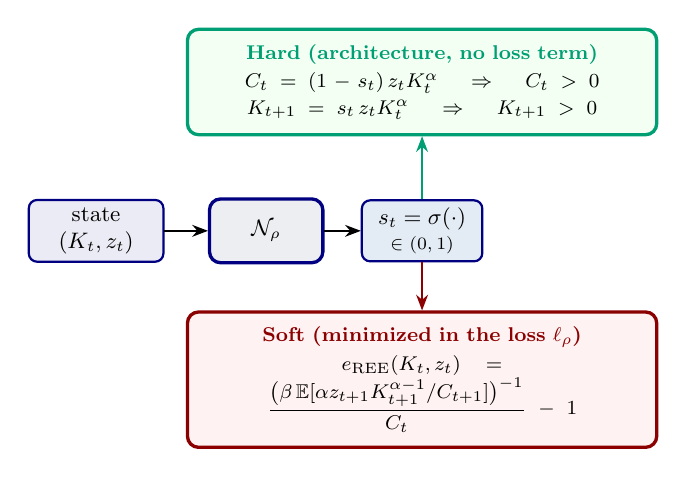
\begin{tikzpicture}[scale=0.90, transform shape,
    io/.style={rectangle, draw=uzhblue, thick, rounded corners=3pt, fill=uzhblue!8,
               minimum width=1.9cm, minimum height=0.8cm, font=\small, align=center, inner sep=3pt},
    dnn/.style={rectangle, draw=uzhblue, very thick, rounded corners=4pt, fill=uzhgreylight,
               minimum width=1.6cm, minimum height=0.9cm, font=\small\bfseries, align=center},
    sig/.style={rectangle, draw=uzhblue, thick, rounded corners=3pt, fill=softblue!15,
               minimum width=1.7cm, minimum height=0.8cm, font=\small, align=center, inner sep=3pt},
    hard/.style={rectangle, draw=softgreen, very thick, rounded corners=4pt, fill=green!5,
               text width=6.2cm, font=\footnotesize, align=center, inner sep=6pt},
    soft/.style={rectangle, draw=darkred, very thick, rounded corners=4pt, fill=red!5,
               text width=6.2cm, font=\footnotesize, align=center, inner sep=6pt},
    arr/.style={-{Stealth[length=2mm]}, thick}
]
    % Center spine: state -> N_rho -> sigmoid(s_t)
    \node[io]  (x)  at (0,0) {state\\$(K_t,z_t)$};
    \node[dnn] (nn) at (2.4,0) {$\mathcal{N}_\rho$};
    \node[sig] (s)  at (4.6,0) {$s_t=\sigma(\cdot)$\\[-1pt]{\scriptsize $\in(0,1)$}};
    \draw[arr] (x)  -- (nn);
    \draw[arr] (nn) -- (s);

    % Hard constraints (top, green)
    \node[hard] (H) at (4.6, 2.1)
        {\textbf{\textcolor{softgreen}{Hard (architecture, no loss term)}}\\[2pt]
         $C_t = (1-s_t)\,z_tK_t^\alpha \quad\Rightarrow\quad C_t>0$ \\[1pt]
         $K_{t+1} = s_t\,z_tK_t^\alpha \quad\Rightarrow\quad K_{t+1}>0$};
    \draw[arr, softgreen, thick] (s.north) -- (H.south);

    % Soft residual (bottom, red)
    \node[soft] (S) at (4.6,-2.1)
        {\textbf{\textcolor{darkred}{Soft (minimized in the loss $\ell_\rho$)}}\\[2pt]
         $e_{\mathrm{REE}}(K_t,z_t) = \dfrac{\bigl(\beta\,\mathbb{E}[\alpha z_{t+1}K_{t+1}^{\alpha-1}/C_{t+1}]\bigr)^{-1}}{C_t}\,-\,1$};
    \draw[arr, darkred, thick] (s.south) -- (S.north);
\end{tikzpicture}
\end{center}

\vspace{-0.25em}
{\footnotesize
\emphc{Why bother?} A softplus head on $C_t$ alone would secure $C_t\!>\!0$ but could push $K_{t+1}\!<\!0$.  The sigmoid-savings head removes \emph{both} failure modes before training starts.  Only the genuinely non-closed-form condition, the Euler equation, enters the loss.}
\end{frame}
\begin{frame}{Choice of Training Loss: Six Kernels}
\footnotesize
The loss kernel is a \emphc{modeling decision}, not a default.  Same Euler residual $r$, same network, same data, only the reduction $r\!\mapsto\!\ell$ changes:

\vspace{0.4em}
\begin{center}
\renewcommand{\arraystretch}{1.15}
\setlength{\tabcolsep}{4pt}
\begin{tabular}{@{}lll@{}}
\toprule
\textbf{Kernel} & \textbf{Formula} & \textbf{Character} \\
\midrule
MSE      & $\tfrac1B\sum r^2$                                & quadratic; canonical default \\
MAE      & $\tfrac1B\sum |r|$                                 & constant gradient $\Rightarrow$ \emphc{stalls at small $|r|$} \\
Huber    & quad.\ for $|r|\!\le\!\delta$, linear above       & robust hybrid, but \emphc{kink at $|r|{=}\delta$} \\
Quantile & pinball at $\tau{=}0.9$                            & trains the upper $\tau$-quantile only \\
CVaR     & mean of top $10\%$ of $|r|$                        & explicitly trains the worst-case states \\
\textbf{LogCosh} & $\tfrac1B\sum\log\cosh(r)$                   & $C^\infty$: $\tfrac12 r^2$ near $0$, $|r|{-}\log 2$ in tails, \emphc{no kink} \\
\bottomrule
\end{tabular}
\end{center}

\vspace{0.6em}
{\scriptsize Same Brock--Mirman model, full depreciation so $s^\star = \alpha\beta$ is in closed form; same network (2$\times$32 swish, sigmoid head); same Adam optimizer; same CRN training stream.  Six runs differ \emph{only} in the reduction applied to the residual vector.}
\end{frame}

\begin{frame}{Loss Kernels: Convergence on Brock--Mirman}
\begin{center}

\includegraphics[width=0.98\linewidth]{figures/loss_kernel_convergence.png}
\end{center}

\vspace{0.2em}
{\footnotesize Mean / $p_{90}$ / $p_{99}$ of the absolute relative Euler error $|r|$ on a fixed evaluation grid, vs.\ training episode (log scale, 5000 episodes per kernel).  \emphc{LogCosh and MSE} reach the lowest mean residual.  \emphc{Huber and CVaR} produce the narrowest tail.  \emphc{MAE stalls} at a noise floor.}
\end{frame}

\begin{frame}{Loss-Kernel Comparison: What to Take Away}
\scriptsize
\begin{itemize}\itemsep1.5pt
    \item \emphc{LogCosh converges most smoothly:} the only $C^\infty$ kernel that is MSE-like near $r=0$ \emph{and} MAE-like in the tails, no kink anywhere.  Lowest-risk default when the residual distribution is unknown.
    \item \emphc{MAE stalls} at a noise floor: constant gradient magnitude prevents smaller steps as residuals shrink.
    \item \emphc{Huber is robust} but its kink at $|r|{=}\delta$ can introduce small oscillations.
    \item \emphc{Quantile and CVaR} narrow $p_{99}$ at the cost of mean residual.  Use them when worst-case policy quality matters (binding constraints, rare-but-consequential states, regulatory back-tests).
    \item \emphc{Evaluate on the economic metric}~---~Euler error along simulated paths, in CE-welfare-loss units~---~not on the training loss itself.  The CE ranking is generally not the training-loss ranking.
\end{itemize}

\vspace{0.4em}
\begin{exampleblock}{Practical default}
\textbf{MSE} for smooth problems; \textbf{LogCosh} as a drop-in that is more forgiving with heavy-tailed residuals; \textbf{Huber / Quantile / CVaR} when the worst-case state matters.
\end{exampleblock}

\vspace{0.2em}
{\scriptsize Companion notebook: \texttt{lecture\_09\_B08\_05\_StochasticBM\_LossComparison.ipynb}.}
\end{frame}
\begin{frame}{Data Parallelism for DEQNs}
\textbf{Idea:} distribute training data across \emphc{multiple workers} (GPUs/CPUs).

\vspace{0.4em}
\begin{center}
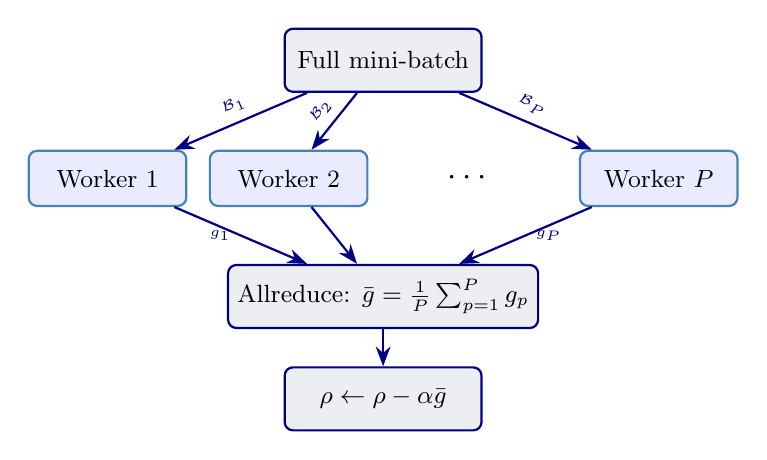
\begin{tikzpicture}[
    mlstep/.style={rectangle, draw=uzhblue, thick, fill=uzhgreylight,
        minimum width=2.5cm, minimum height=0.8cm, font=\small,
        rounded corners=3pt},
    worker/.style={rectangle, draw=softblue, thick, fill=blue!8,
        minimum width=2.0cm, minimum height=0.7cm, font=\small,
        rounded corners=3pt},
    arr/.style={-{Stealth[length=2.5mm]}, thick, uzhblue}
]
    \node[mlstep] (data) at (0,0) {Full mini-batch};
    \node[worker] (w1) at (-3.5,-1.5) {Worker 1};
    \node[worker] (w2) at (-1.2,-1.5) {Worker 2};
    \node[font=\large] (dots) at (1.1,-1.5) {$\cdots$};
    \node[worker] (wP) at (3.5,-1.5) {Worker $P$};

    \node[mlstep] (grad) at (0,-3.0) {Allreduce: $\bar{g} = \frac{1}{P}\sum_{p=1}^P g_p$};
    \node[mlstep] (upd) at (0,-4.3) {$\rho \leftarrow \rho - \alpha \bar{g}$};

    \draw[arr] (data) -- (w1) node[midway, above, font=\tiny, sloped] {$\mathcal{B}_1$};
    \draw[arr] (data) -- (w2) node[midway, above, font=\tiny, sloped] {$\mathcal{B}_2$};
    \draw[arr] (data) -- (wP) node[midway, above, font=\tiny, sloped] {$\mathcal{B}_P$};

    \draw[arr] (w1) -- (grad) node[midway, left, font=\tiny] {$g_1$};
    \draw[arr] (w2) -- (grad);
    \draw[arr] (wP) -- (grad) node[midway, right, font=\tiny] {$g_P$};

    \draw[arr] (grad) -- (upd);
\end{tikzpicture}
\end{center}

\vspace{0.2em}
{\small Implemented via \textbf{Horovod}/MPI. Each worker computes a local gradient; \emphc{allreduce} averages them.}
\end{frame}

% --- Slide 29: Parallelization Scheme ---
\begin{frame}{DEQN Parallelization Scheme}
\begin{center}
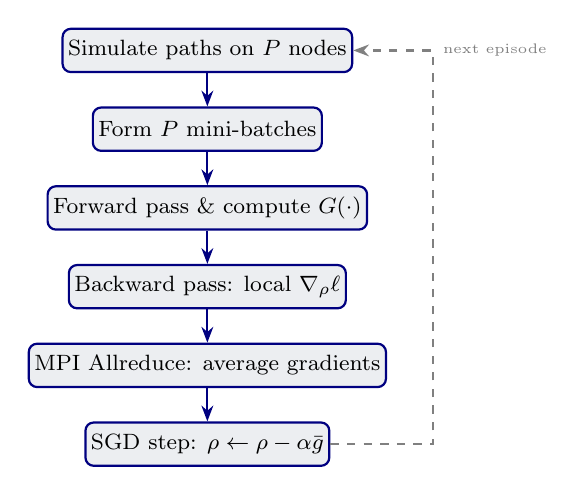
\begin{tikzpicture}[
    mlstep/.style={rectangle, draw=uzhblue, thick, fill=uzhgreylight,
        minimum width=2.8cm, minimum height=0.55cm, font=\footnotesize,
        rounded corners=3pt, inner sep=2pt},
    arr/.style={-{Stealth[length=2mm]}, thick, uzhblue}
]
    \node[mlstep] (sim) at (0,0) {Simulate paths on $P$ nodes};
    \node[mlstep] (mb) at (0,-1.0) {Form $P$ mini-batches};
    \node[mlstep] (fwd) at (0,-2.0) {Forward pass \& compute $G(\cdot)$};
    \node[mlstep] (bwd) at (0,-3.0) {Backward pass: local $\nabla_\rho \ell$};
    \node[mlstep] (all) at (0,-4.0) {MPI Allreduce: average gradients};
    \node[mlstep] (step) at (0,-5.0) {SGD step: $\rho \leftarrow \rho - \alpha \bar{g}$};

    \draw[arr] (sim) -- (mb);
    \draw[arr] (mb) -- (fwd);
    \draw[arr] (fwd) -- (bwd);
    \draw[arr] (bwd) -- (all);
    \draw[arr] (all) -- (step);

    \draw[arr, dashed, gray] (step.east) -- ++(1.3,0) |- (sim.east)
        node[midway, right, font=\tiny, text=gray] {next episode};
\end{tikzpicture}
\end{center}

{\small Communication cost $\sim \mathcal{O}(|\rho|)$ per step, independent of data size.}
\end{frame}

% --- Slide 30: Scalability ---
\begin{frame}{Illustrative Scaling Pattern}
\begin{center}
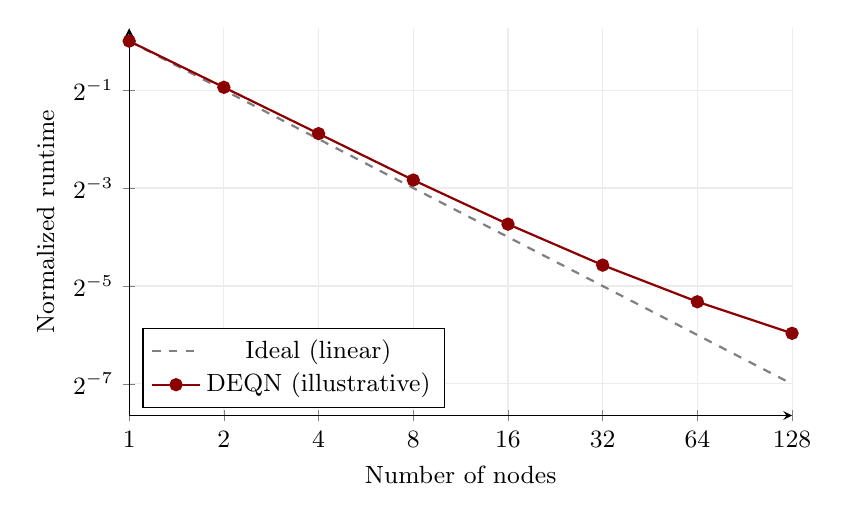
\begin{tikzpicture}
\begin{axis}[
    width=10cm, height=6.5cm,
    xlabel={Number of nodes},
    ylabel={Normalized runtime},
    xlabel style={font=\small},
    ylabel style={font=\small},
    tick label style={font=\small},
    xmode=log, ymode=log,
    log basis x=2, log basis y=2,
    xmin=1, xmax=128, ymin=0.005, ymax=1.2,
    grid=major, grid style={gray!15},
    legend style={font=\small, at={(0.02,0.02)}, anchor=south west},
    axis lines=left,
    xtick={1,2,4,8,16,32,64,128},
    xticklabels={1,2,4,8,16,32,64,128},
]
    % Ideal scaling
    \addplot[thick, dashed, gray, domain=1:128, samples=8]
        {1/x};
    \addlegendentry{Ideal (linear)}

    % Realized scaling (slightly worse)
    \addplot[thick, darkred, mark=*, mark size=2pt]
        coordinates {
            (1, 1.0) (2, 0.52) (4, 0.27) (8, 0.14)
            (16, 0.075) (32, 0.042) (64, 0.025) (128, 0.016)
        };
    \addlegendentry{DEQN (illustrative)}
\end{axis}
\end{tikzpicture}
\end{center}

{\small Schematic message only: synchronous data parallelism is often close to linear for moderate worker counts; large clusters become increasingly communication-limited.}
\end{frame}
\begin{frame}{Hands-on Notebooks}
\textbf{Four notebooks} accompany this lecture:

\vspace{0.4em}
\begin{enumerate}\itemsep2pt
    \item \texttt{01\_Brock\_Mirman\_1972\_DEQN.ipynb}\\
    {\small Deterministic Brock--Mirman, \emphc{exogenous uniform sampling} of states.}

    \item \texttt{02\_Brock\_Mirman\_Uncertainty\_DEQN.ipynb}\\
    {\small Stochastic Brock--Mirman ($\varrho > 0$, $\sigma_z > 0$), \emphc{simulation-based sampling} on the ergodic set.}

    \item \texttt{03\_DEQN\_Exercises\_Blanks.ipynb} (exercises, blank template for student populate)

    \item \texttt{04\_DEQN\_Exercises\_Solutions.ipynb} (exercises, solved)
\end{enumerate}

\vspace{0.3em}
{\footnotesize Notebooks 01--02 illustrate the sampling progression: uniform random $\to$ simulated trajectories.  Notebooks 03--04 add KKT multipliers + Fischer--Burmeister + the 6-period OLG structure previewed on the previous slide.}

\vspace{0.4em}
All notebooks are in the course repository.
\end{frame}
\begin{frame}{}
\begin{columns}[c]
\column{0.45\textwidth}
\begin{center}
{\Huge \textcolor{uzhblue}{\textbf{Questions?}}}

\vspace{1.0cm}
{\large Simon Scheidegger}\\[4pt]
{\small HEC, University of Lausanne}\\[4pt]
\url{https://sischei.github.io}

\vspace{0.6cm}
{\small Materials:~~\url{https://github.com/sischei/Deep_Learning_for_Solving_And_Estimating_Dynamic_Economic_Models}}
\end{center}

\column{0.45\textwidth}
\begin{center}
\textbf{Next up:}\\[6pt]
{\large DEQN Exercises}\\[12pt]
\end{center}
\end{columns}
\end{frame}

\end{document}
